\documentclass[tikz,border=5pt]{standalone}
\usepackage{tikz}
\usetikzlibrary{positioning,calc,arrows.meta}

% =========================
% Customization
% =========================
\newcommand{\InputTopLabel}{$x_1$}
\newcommand{\InputBottomLabel}{$x_n$}
\newcommand{\LinearTerm}{$\displaystyle\sum_{i=1}^{n} w_i x_i + b$}
\newcommand{\ActivationTerm}{$\sigma(\cdot)$}
\newcommand{\OutputTerm}{$\sigma\left(\sum_{i=1}^{n} w_i x_i + b\right)$}
\def\NeuronSize{2.2cm}
\def\InputVerticalOffset{1.1cm}
\def\OutputOffset{3.2cm}

\tikzset{
  signal/.style={->,>=Latex,line width=0.7pt},
  neuron/.style={
    circle,
    draw=black,
    minimum size=\NeuronSize,
    line width=0.8pt
  }
}

\begin{document}
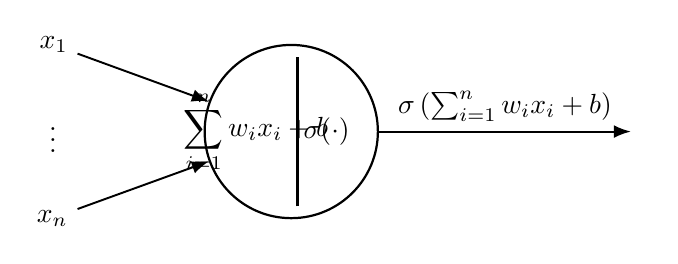
\begin{tikzpicture}
  \node[neuron] (neuron) at (0,0) {};
  \node[align=center] at ([xshift=-0.45cm]neuron.center) {\LinearTerm};
  \node at ([xshift=0.45cm]neuron.center) {\ActivationTerm};

  % Separator between affine transformation and activation.
  \draw[line width=0.8pt]
    ([xshift=0.08cm,yshift=-0.95cm]neuron.center) --
    ([xshift=0.08cm,yshift=0.95cm]neuron.center);

  \node[left=1.6cm of neuron, yshift=\InputVerticalOffset] (x1) {\InputTopLabel};
  \node[left=1.6cm of neuron, yshift=-\InputVerticalOffset] (xn) {\InputBottomLabel};
  \node at ($(x1)!0.5!(xn)$) {\(\vdots\)};

  \node[right=\OutputOffset of neuron] (out) {};

  \draw[signal] (x1) -- (neuron);
  \draw[signal] (xn) -- (neuron);
  \draw[signal] (neuron) -- node[above,midway] {\OutputTerm} (out);
\end{tikzpicture}
\end{document}
